\Problem
{\lr{RIL info via adb}}
{
برای حل این سوال ابتدا بایستی حالت
\lr{Developer Mode}
را در تلفن همراه اندرویدی ایجاد کنیم.
برای اینکار به قسمت
\lr{Setting}
می‌رویم.
سپس در قسمت
\lr{About Phone}
فیلد
\lr{Build Number}
را پیدا می‌کنیم و هفت مرتبه روی آن ضربه می‌زنیم تا این حالت فعال شود.
در تنظیمات آن حالت
\lr{USB Debugging}
را نیز فعال می‌کنیم.
\begin{figure}[H]
    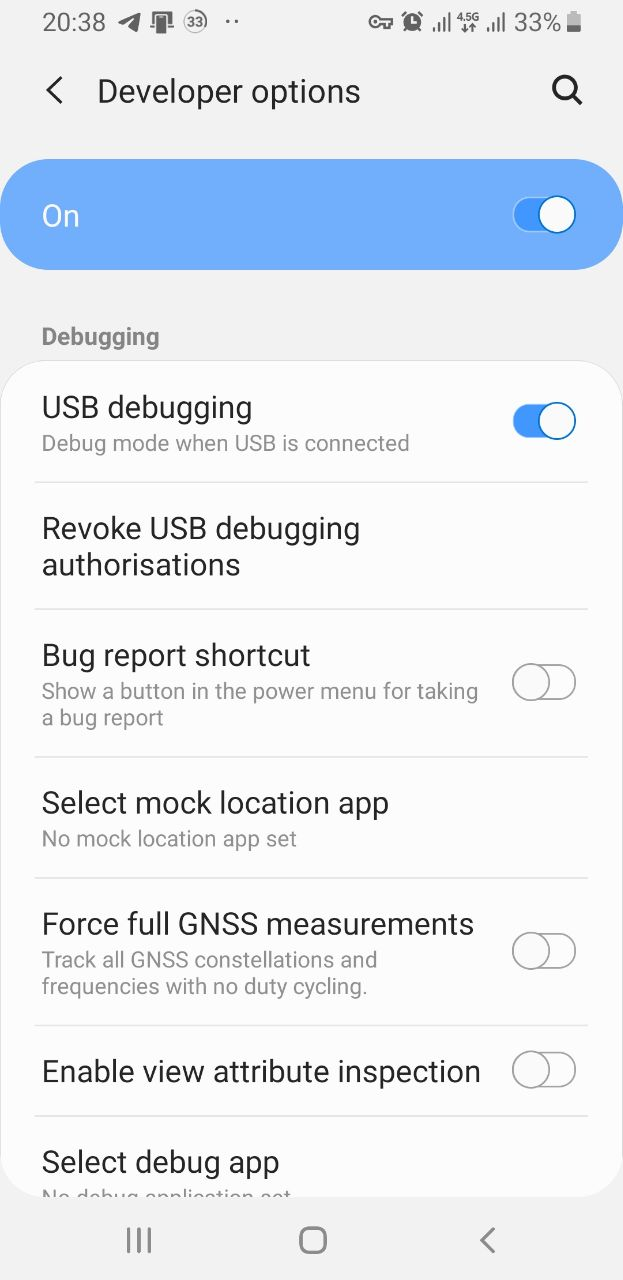
\includegraphics[width=7cm]{Images/Android.jpg}
    \centering
    \caption{تنظیمات داخل گوشی}
\end{figure}
\newpage
سپس برنامه
\lr{adb}
را دانلود می‌کنیم و در محلی آن را استخراج می‌کنیم.
\begin{figure}[H]
    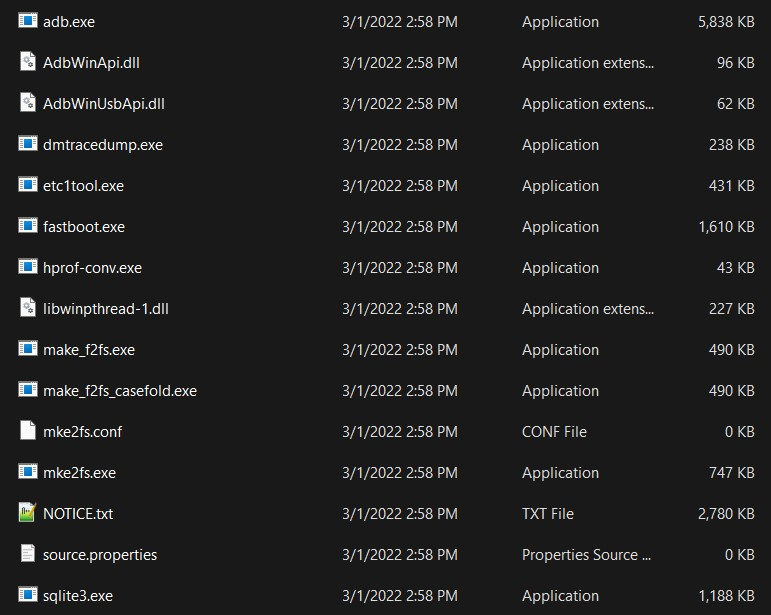
\includegraphics[width=10cm]{Images/adb.jpg}
    \centering
    \caption{فایل‌های \lr{adb}}
\end{figure}

تلفن همراه را با کابل مناسب به لپتاپ متصل می‌کنیم. سپس دستورات زیر را وارد می‌کنیم.

\begin{center}
    \lr{adb devices}
\end{center}
\begin{figure}[H]
    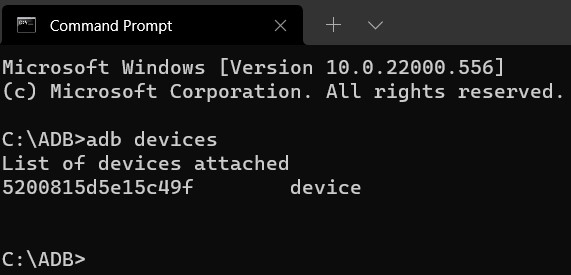
\includegraphics[width=10cm]{Images/devices.jpg}
    \centering
    \caption{لیست دستگاه‌ها}
\end{figure}
\newpage
سپس دستور زیر را وارد می‌کنیم تا اطلاعات
\lr{RIL}
را مشاهده کنیم.
\begin{center}
    \lr{adb logcat -b radio}
\end{center}
\begin{figure}[H]
    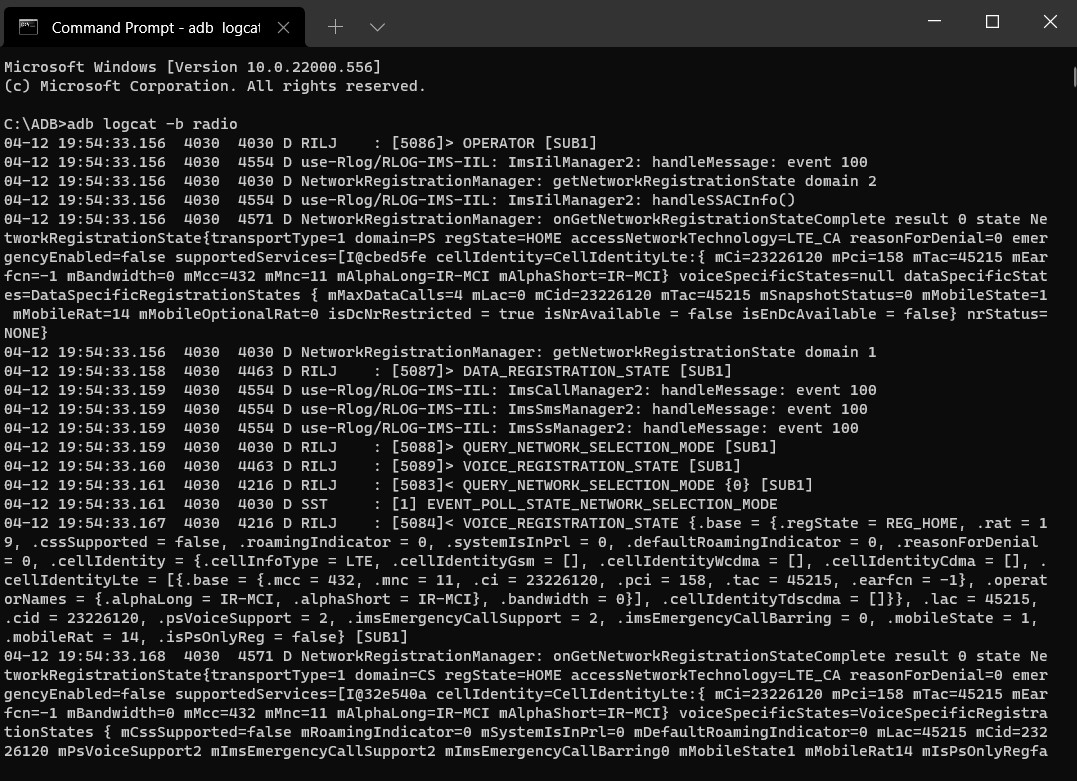
\includegraphics[width=15cm]{Images/logs.jpg}
    \centering
    \caption{اطلاعات}
\end{figure}
}
